\documentclass[journal,12pt,onecolumn]{IEEEtran}
\usepackage{cite}
\usepackage{graphicx}
\usepackage{amsmath,amssymb,amsfonts,amsthm}
\usepackage{algorithmic}
\usepackage{textcomp}
\usepackage{xcolor}
\usepackage{txfonts}
\usepackage{listings}
\usepackage{enumitem}
\usepackage{mathtools}
\usepackage{gensymb}
\usepackage{comment}
\usepackage[breaklinks=true]{hyperref}
\usepackage{tkz-euclide} 
\usepackage{caption}
\usepackage{listings}
\usepackage{gvv}                                        
\usepackage[latin1]{inputenc} 
\usetikzlibrary{arrows.meta, positioning}
\usepackage{xparse}
\usepackage{color}                                            
\usepackage{array}                                            
\usepackage{longtable}                                       
\usepackage{calc}                                             
\usepackage{multirow}
\usepackage{multicol}
\usepackage{hhline}                                           
\usepackage{ifthen}                                           
\usepackage{lscape}
\usepackage{tabularx}
\usepackage{array}
\usepackage{float}
\newtheorem{theorem}{Theorem}[section]
\newtheorem{problem}{Problem}
\newtheorem{proposition}{Proposition}[section]
\newtheorem{lemma}{Lemma}[section]
\newtheorem{corollary}[theorem]{Corollary}
\newtheorem{example}{Example}[section]
\newtheorem{definition}[problem]{Definition}
\newcommand{\BEQA}{\begin{eqnarray}}
\newcommand{\EEQA}{\end{eqnarray}}
\usepackage{float}
\theoremstyle{remark}
\usepackage{circuitikz}
\usepackage{tikz}\title{}
\title{\Huge MN:MINING ENGINEERING}
\author{Vaishnavi Ramkrishna Anantheertha-EE25BTECH11059}
\begin{document}
\maketitle

\section*{Q.1--Q.25 carry one mark each}
\begin{enumerate}
\item Ascensionally ventilated coal mine inclines ideally should have higher methane layering number when compared to descensionally ventilated inclines. The reason is $\colon$

\hfill\brak{GATE\ MN\ 2010}
\begin{enumerate}
\item In ascensionally ventilated incline, density of air is higher
\item Ascensionally ventilated incline creates conditions for improved turbulent mixing of methane layer
\item Methane drainage is not practiced in ascensionally ventilated incline
\item Descensionally ventilated incline creates conditions for improved turbulent mixing of methane layer
\end{enumerate}
\item A coolant is a desirable component in the design of a Self-Contained Breathing Apparatus since $\colon$

\hfill\brak{GATE\ MN\ 2010}
\begin{multicols}{2}
\begin{enumerate}
\item Surroundings can be hot and humid during rescue
\item A rescue worker generates large amount of metabolic heat
\item Exhaled air CO\textsubscript{2} absorption is an exothermic reaction
\item Exhaled air water vapour has to be condensed
\end{enumerate}
\end{multicols}
\item  Determine the correctness or otherwise of the following Assertion \sbrak{a} and the Reason \sbrak{r} $\colon$
\vspace{0.5em}
\noindent

\textbf{Assertion \sbrak{a} $\colon$} Both intake and return side stoppings must be closed simultaneously in the event of sealing off a coal mine panel with explosion hazard following a fire.

\vspace{0.5em}
\noindent
\textbf{Reason \sbrak{r} $\colon$} By continuously ventilating the area till simultaneous closure of the stoppings, the possibility of an explosion hazard due to gas build-up is avoided.
\vspace{1em}

\hfill\brak{GATE\ MN\ 2010}    
\begin{enumerate}
    \item \sbrak{a} is true but \sbrak{r} is false
    \item Both \sbrak{a} and \sbrak{r} are true and \sbrak{r} is the correct reason for \sbrak{a}
    \item Both \sbrak{a} and \sbrak{r} are true and \sbrak{r} is not the correct reason for \sbrak{a}
    \item Both \sbrak{a} and \sbrak{r} are false

\end{enumerate}
\item In a Cartesian coordinate system the vertices of a triangular plate are given by $\brak{-2, 1}$,$\brak{3, 4}$,and $\brak{-4, -8}$.The coordinates of the centre of gravity of the plate are.

\hfill\brak{GATE\ MN\ 2010}
\begin{multicols}{4}
\begin{enumerate}
\item $\brak{3,4}$
\item $\brak{7,12}$ 
\item $\brak{-1,-1}$
\item $\brak{-3,-4}$
\end{enumerate}
\end{multicols}
\item An air quality parameter required to be monitored under the Indian National Ambient Air Quality Standards is

\hfill\brak{GATE\ MN\ 2010} 
\begin{multicols}{4}
\begin{enumerate}
\item $As$
\item $Pb$
\item $Hg$
\item Silica
\end{enumerate}
\end{multicols}
\item In an underground coal mine, a freshly exposed roof can be supported by a temporary support in the form of

\hfill\brak{GATE\ MN\ 2010}
\begin{multicols}{4}
\begin{enumerate}
\item triangular chocks
\item screw props 
\item safari supports
\item hydraulic props
\end{enumerate}
\end{multicols}
\item At a surface mine office the independent Sound Pressure Levels $\brak{SPL}$ measured in dB(A) on account of $3$ drill machines are $85$,$88$ and $85$. If all the three machines work simultaneously, the combined SPL,in dB(A), is

\hfill\brak{GATE\ MN\ 2010}
\begin{multicols}{4}
\begin{enumerate}
\item $91$
\item $90$ 
\item $92$
\item $94$
\end{enumerate}
\end{multicols}
\item The backsight reading on a bench mark of RL $100.0$ m is $1.45$ m. If the inverse staff reading on a foresight is $2.23$ m, the RL of the staff station in m is

\hfill\brak{GATE\ MN\ 2010}
\begin{multicols}{4}
\begin{enumerate}
\item $105.13$
\item $103.68$ 
\item $100.78$
\item $98.55$
\end{enumerate}
\end{multicols}
\item For a mine of production per year, the total cost of production is given by $at^2 + b$. The revenue from sale is given by ct. If a, b and c, are constants, the breakeven value of t is

\hfill\brak{GATE\ MN\ 2010}
  \begin{multicols}{2}
  \begin{enumerate}
    \item $\displaystyle \frac{c \pm \sqrt{c^2 - 4ab}}{2a}$
    \item $\displaystyle \frac{\sqrt{c^2 - 4ab}}{2a}$
    \item $\displaystyle \frac{-c \pm \sqrt{c^2 - 4ab}}{2a}$
    \item $\displaystyle \frac{c \pm \sqrt{c^2 + 4ab}}{2a}$
\end{enumerate}
  \end{multicols}
\item The value of the\[\lim_{x \to 1} \frac{\,1 - x^{-1/3}\,}{\,1 - x^{-2/3}\,}\] is

\hfill\brak{GATE\ MN\ 2010}
\begin{multicols}{4}
\begin{enumerate}
\item $\infty$
\item $1$
\item $0$
\item $\frac{1}{2}$
\end{enumerate}
\end{multicols}
\item Two determinants of order n are multiplied. The order of the resultant determinant is

\hfill\brak{GATE\ MN\ 2010}
\begin{multicols}{4}
\begin{enumerate}
\item $n$
\item $2n$
\item $n^2$
\item $n/2$
\end{enumerate}
\end{multicols}
\item The partial differential equation,$r\frac{\partial \theta}{\partial r}=constant$,is a solution for

\hfill\brak{GATE\ MN\ 2010}
\begin{multicols}{2}
\begin{enumerate}
\item $\quad \frac{\partial^2 \theta}{\partial r^2} \;-\; \frac{1}{r}\,\frac{\partial \theta}{\partial r} = 0$
\item $\quad \frac{\partial^2 \theta}{\partial r^2} + \frac{\partial \theta}{\partial r} = 0$
\item $\quad r^2 \frac{\partial^2 \theta}{\partial r^2}
         + r \frac{\partial \theta}{\partial r} = 0$
\item $\quad \frac{\partial^2 \theta}{\partial r^2} \;+\; \frac{1}{r}\,\frac{\partial \theta}{\partial r} = 0$
\end{enumerate}
\end{multicols}
\item In Mohr-Coulomb failure criterion, the ratio of the uniaxial compressive strength to the tensile strength is

\hfill\brak{GATE\ MN\ 2010}
\begin{multicols}{2}
\begin{enumerate}
  \item $\dfrac{1 + \sin\phi}{1 - \sin\phi}$
  \item $\dfrac{1 - \sin\phi}{1 + \sin\phi}$
  \item $\dfrac{C\,(1 + \sin\phi)}{1 - \sin\phi}$
  \item $\dfrac{2C\,(1 + \sin\phi)}{1 - \sin\phi}$
\end{enumerate}
\end{multicols}

 \item The average Young's modulus and Poisson's ratio values of a limestone sample are $60 \times 10^3$ MPa and $0.3$ respectively. The shear modulus in MPa is
\hfill\brak{GATE\ MN\ 2010}
\begin{multicols}{4}
\begin{enumerate}
\item $23.07$
\item $230.7$
\item $2307.0$
\item $23070.0$
\end{enumerate}
\end{multicols}

\item The angle of draw in a trough subsidence helps in determining the

\hfill\brak{GATE\ MN\ 2010}
\begin{multicols}{2}
\begin{enumerate}
\item maximum subsidence
\item extent of surface subsidence
\item plane of fracture
\item critical width of the opening
\end{enumerate}
\end{multicols}

\item Recapping a winding rope is done to

\hfill\brak{GATE\ MN\ 2010}
\begin{enumerate}
\item increase the flexural strength of the rope
\item increase the flexibility of the rope
\item remove a portion of the rope subjected to deterioration
\item  prevent the rope from excessive rusting
\end{enumerate}

\item Match the following
\vspace{0.5em}

\hfill\brak{GATE\ MN\ 2010}
\begin{table}[H]
  \centering
  \caption{Match The Following}
  \begin{tabular}{>{\bfseries}l l}
Specification & Outer Diameter in mm \\
P. AW & p. 34.9 \\
Q. BW & q. 44.4 \\
R. EW & r. 54.0 \\
S. NW & s. 66.7 \\
\end{tabular}


  \label{tab:Table1}
\end{table}
\begin{multicols}{2}
\begin{enumerate}
\item P-r; Q-q; R-s; S-p  
\item P-r; Q-p; R-s; S-q  
\item P-q; Q-r; R-p; S-s  
\item P-q; Q-r; R-s; S-p  
\end{enumerate}
\end{multicols}

\item Payback period is time required

\hfill\brak{GATE\ MN\ 2010}
\begin{enumerate}
\item for the cash income from a project to get back the initial cash investment  
\item from the start of the project to the time to recover the total initial investment  
\item from the start of the project to the start of production  
\item to the period during which internal rate of return is generated  
\end{enumerate}

\item For electric signaling systems in underground coal mines, the statement that is NOT true is

\hfill\brak{GATE\ MN\ 2010}
\begin{enumerate}
\item all signaling equipment must be intrinsically safe
\item the signaling circuit must be connected to ground
\item the source of current should be an approved dry battery
\item DC bells or retays when connected in parallel should be supplied from a single source of current
\end{enumerate}
\item  A ladder of weight 50 N rests against a frictionless wall and floor as shown in the figure. A horizontal string ties the base of the ladder to the wall. The tension in the string in N is

\hfill\brak{GATE\ MN\ 2010}
\begin{figure}[H]
  \centering
  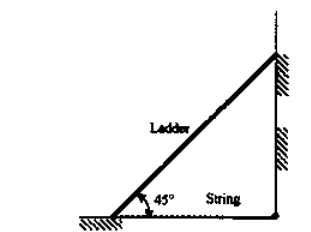
\includegraphics[width=0.4\columnwidth]{figs/ladder.png}
  \caption{Illustration of the ladder mechanism.}
  \label{fig:ladder}
\end{figure}
\begin{multicols}{4}
\begin{enumerate}
\item $100$
\item $50$
\item $72$
\item $25$
\end{enumerate}
\end{multicols}
\item The mean and the standard deviation of the grade of iron ore in a deposit are $62$\% and $5$\%
respectively. The coefficient of variation of the grade in \% is

\hfill\brak{GATE\ MN\ 2010}
\begin{multicols}{4}
\begin{enumerate}
\item $24.8$
\item $12.4$
\item $8.0$
\item $4.0$
\end{enumerate}
\end{multicols}
\item The variance of failure time $\brak{time\ to\ failures}$ of an electric motor in shovel is $1600$ $hr^2$. If the failure time follows an exponential distribution, the expected failure time in hr is

\hfill\brak{GATE\ MN\ 2010}
\begin{multicols}{4}
\begin{enumerate}
\item $40$
\item $80$
\item $800$
\item $1600$
\end{enumerate}
\end{multicols}
\item Match the following for standard diamond drill rods.
\begin{table}[H]
  \centering
  \caption{Match The Following}
  \begin{table}[ht]
\centering
\begin{tabular}{|l|l|}
\hline
\textbf{Column I} & \textbf{Column II} \\ \hline
P. Hydraulic Conductivity   & 1. Upper limit of moisture available to plant \\ \hline
Q. Permeability            & 2. All soil pores are filled with water         \\ \hline
R. Viscosity               & 3. Soil capillarity                            \\ \hline
S. Surface Tension         & 4. Properties of fluid as well as soil          \\ \hline
T. Saturation Capacity     & 5. Property of the medium                      \\ \hline
U. Field Capacity          & 6. Internal friction that brings about resistance to flow \\ \hline
\end{tabular}
\end{table}
  \label{tab:table3}
\end{table}
\vspace{0.5em}
\hfill\brak{GATE\ MN\ 2010}


\vspace{0.5em}

\begin{multicols}{2}
\begin{enumerate}
\item  1-a; 2-c; 3-d; 4-b  
\item 1-c; 2-b; 3-d; 4-a  
\item  1-d; 2-a; 3-d; 4-c  
\item 1-d; 2-c; 3-b; 4-a
  
\end{enumerate}
\end{multicols}
\item A cage weighing $12000$ kg is raised by four chains each making an angle of $30^\circ$ with the vertical.The tension in each chain in kN is

\hfill\brak{GATE\ MN\ 2010}
\begin{multicols}{4}
\begin{enumerate}
\item $41$
\item $34$
\item $25$
\item $20$
\end{enumerate}
\end{multicols}
\item The relationship between the drawbar puil and the speed for different gears of a self propelling vehicle is represented by

\hfill\brak{GATE\ MN\ 2010}
\begin{figure}[H]
  \centering
  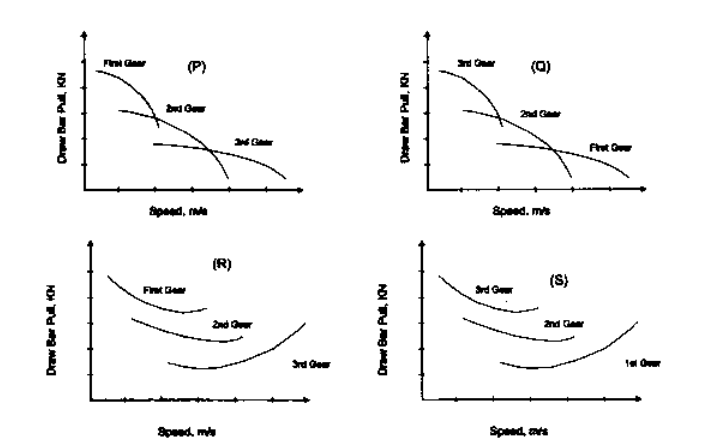
\includegraphics[width=0.4\columnwidth]{figs/graphs.png}
  \caption{Graphical illustrations}
  \label{fig:graphs}
\end{figure}
\begin{multicols}{4}
\begin{enumerate}
\item Q
\item S
\item R
\item P
\end{enumerate}
\end{multicols}

\section*{Q.26--Q.55 carry one mark each}
\item A flammable mixture has $70$ \% $CH_4$, and $30$\% $CO$. The lower flammability limits for these gases are
$5$\% and $13$\% respectively. For the mixture, the lower flammability limit in \% is

\hfill\brak{GATE\ MN\ 2010}
\begin{multicols}{4}
\begin{enumerate}
\item $6.13$
\item $8.72$
\item $10.25$
\item $12.16$
\end{enumerate}
\end{multicols}
\item The volume of tetrahedron with vertices at $\brak{0,0,0}$, $\brak{1,0,0}$, $\brak{0,1,0}$ and $\brak{0,0,1}$ is

\hfill\brak{GATE\ MN\ 2010}
\begin{multicols}{4}
\begin{enumerate}
\item $\frac{1}{2}$
\item $\frac{1}{4}$
\item $\frac{1}{6}$
\item $\frac{1}{8}$
\end{enumerate}
\end{multicols}
\item  A balanced winder raises $3000$ tonnes per day from a depth of $500$ m The payload of the winding cage is $7$ tonnes. The energy consumed per day in kWh at $70$\% winder efficiency is

\hfill\brak{GATE\ MN\ 2010}
\begin{multicols}{4}
\begin{enumerate}
\item $6030$
\item $5840$
\item $5750$
\item $5630$
\end{enumerate}
\end{multicols}

\item A truss is loaded as shown in the figure. The force in the member AC is

\hfill\brak{GATE\ MN\ 2010}
\begin{figure}[H]
  \centering
  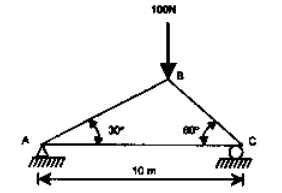
\includegraphics[width=0.4\columnwidth]{figs/truss.png}
  \caption{truss}
  \label{fig:truss}
\end{figure}
\begin{multicols}{2}
\begin{enumerate}
\item tension $75.9$ N
\item compression $43.3$ N
\item tension $43.3$ N
\item compression $75.9$ N
\end{enumerate}
\end{multicols}

\item In the frictionless pulley system shown in the figure, each pulley weighs $20$ N.  
The weight \( W \), in N, that can be lifted by the system under the conditions shown is $\colon$


\hfill\brak{GATE\ MN\ 2010}

\begin{figure}[H]
  \centering
  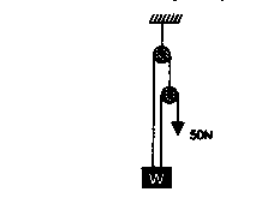
\includegraphics[width=0.4\columnwidth]{figs/pulley.png}
  \caption{Schematic diagram of a pulley system}
  \label{fig:pulley}
\end{figure}
\begin{multicols}{4}
\begin{enumerate}
\item $200$
\item $170$
\item $150$
\item $100$
\end{enumerate}
\end{multicols}

\item A force of $\vec{F} = 50\hat{i} - 50\hat{j} \, \text{N}$ is moved from the origin to the coordinate $\brak{4.0\,\text{m}, 2.0\,\text{m}}$. The work done in the process, in joules, is.


\hfill\brak{GATE\ MN\ 2010}

\begin{multicols}{4}
\begin{enumerate}
\item $75.6$
\item $85.5$
\item $90.2$
\item $100.0$
\end{enumerate}
\end{multicols}

\item The queue of tricks at a crusher plant hopper is known to be M/M/I queue. The probability that
there is no truck to unload is $0.3$.Due to rains the mean service time at the hopper is increased by $30$\%. As a consequence, the expected number of trucks in the queuing system 
\brak{including\ the\ one\ possibly\ unloading} becomes

\hfill\brak{GATE\ MN\ 2010}

\begin{multicols}{4}
\begin{enumerate}
\item $10$
\item $12$
\item $14$
\item $16$
\end{enumerate}
\end{multicols}

\item Pull from an underground tunnel blasting is normally distributed with a mean of $100$ tonnes and variance $100$ $\brak{tonnes}^2$. The probability that the tonnage value from a blast exceeds $110$ is


\hfill\brak{GATE\ MN\ 2010}

\begin{multicols}{4}
\begin{enumerate}
\item $0.60 $
\item $0.80$
\item $0.16$
\item $0.32$
\end{enumerate}
\end{multicols}

\item The feasible region of a LP problem in variables $x$ and $y$ is given by the following constraints \brak{along\ with\ the\ non-negativity\ constraints} 
$y \leq 60$, $x \leq 90$, and $x + y \leq 70$.
The number of corner point feasible solutions for this problem are.
\

\hfill\brak{GATE\ MN\ 2010}

\begin{multicols}{4}
\begin{enumerate}
\item $3$
\item $4$
\item $5$
\item $6$
\end{enumerate}
\end{multicols}

\item The unit cost matrix of a balanced transportation problem is shown below
\begin{table}[H]
  \centering
  \caption{Unit cost matrix}
  \begin{center}
\begin{tabular}{|c|c|c|c|c|c|}
\hline
Mass of particles, g      & 2   & 5   & 7   & 4   & 1    \\
\hline
Mean size of particles, $\mu$m & 350 & 240 & 200 & 150 & 100 \\
\hline
\end{tabular}
\end{center}
  \label{tab:table2}
\end{table}
The transportation cost of the initial basic feasible solution obtained by the North-West corner rule is 

\hfill\brak{GATE\ MN\ 2010}
\begin{multicols}{4}
\begin{enumerate}
\item $1025$
\item $1075$
\item $1130$
\item $1226$
\end{enumerate}
\end{multicols}

\item A high volume air sampler is operated for 8 hours in a mine with the flow rate of air varying from 
$1.5\, \mathrm{m}^3/\mathrm{min}$ to $1.3\, \mathrm{m}^3/\mathrm{min}$. The empty weight of the filter paper is 
$2.30\, \mathrm{g}$ and the final weight is $2.65\, \mathrm{g}$. The mean concentration of the Suspended 
Particulate Matter \brak{SPM} during the study period in $\mu\mathrm{g}/\mathrm{m}^3$ is

\hfill\brak{GATE\ MN\ 2010}
\begin{multicols}{4}
\begin{enumerate}
\item $591$
\item $550$
\item $545$
\item $ 521$
\end{enumerate}
\end{multicols}

\item In an opencast mine shown in the figure below, the coal has a density of $1.4\, \mathrm{tonne}/\mathrm{m}^3$. Assuming
mining operation started from plane $XY$, the operating stripping ratio under the given conditions in 
$\mathrm{m^3}/\mathrm{tonne}$ is

\hfill\brak{GATE\ MN\ 2010}
\begin{figure}[H]
  \centering
  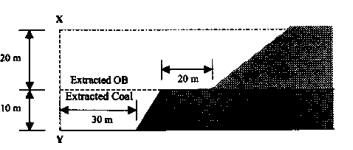
\includegraphics[width=0.4\columnwidth]{figs/37.png}
  \caption{Opencast Mine}
  \label{fig:37}
\end{figure}
\begin{multicols}{4}
\begin{enumerate}
\item $ 2.32$
\item $ 2.47$
\item $ 2.56$
\item $ 2.64$
\end{enumerate}
\end{multicols}

\item A developed panel for a coal seam having an incubation period of 6 months has 32 square pillars 
under extraction, each having a size of $25\,\mathrm{m}$ and a height of $3.0\,\mathrm{m}$. 
The density of coal is $1.4\,\mathrm{tonne/m^3}$. The extraction ratio during depillaring is expected to be $75\%$. 
To depillar the panel within the incubation period, assuming $25$ working days in a month, the production from  the panel in $\mathrm{tonne/day}$ is

\hfill\brak{GATE\ MN\ 2010}
\begin{multicols}{4}
\begin{enumerate}
\item $420$
\item $480$
\item $560$
\item $680$
\end{enumerate}
\end{multicols}

\item A closed traverse ABCDE of perimeter $425\,\mathrm{m}$ has a total error $+0.25\,\mathrm{m}$ in latitude and$-0.44\,\mathrm{m}$ in departure. The precision of traverse is

\hfill\brak{GATE\ MN\ 2010}
\begin{multicols}{4}
\begin{enumerate}
\item $1$ in $556$
\item $1$ in $785$
\item $1$ in $833$
\item $1$ in $1024$
\end{enumerate}
\end{multicols}

\item The value of the given integral is

\[
\int_{\frac{\pi}{5}}^{\frac{\pi}{10}} \frac{\sin x}{\sin x + \cos x} \, dx
\]

\hfill\brak{GATE\ MN\ 2010}
\begin{multicols}{4}
\begin{enumerate}
\item $\dfrac{\sin \frac{\pi}{8}}{10}$
\item $\dfrac{\pi}{10}$
\item $\dfrac{\sin \frac{\pi}{5}}{10}$
\item $\dfrac{3\pi}{10}$
\end{enumerate}
\end{multicols}

\item  The probabilities of hitting a target by A and B are $\frac{1}{3}$ and $\frac{2}{5}$ respectively. A shoots at the target
once, followed by B shooting at the target once. The probability of hitting the target is

\hfill\brak{GATE\ MN\ 2010}
\begin{multicols}{4}
\begin{enumerate}
\item $\frac{2}{15}$
\item $\frac{5}{15}$
\item $\frac{8}{15}$
\item $\frac{9}{15}$
\end{enumerate}
\end{multicols}

\item  The value of k for which the points $\brak{5,5}$,$\brak{k,1}$,$\brak{10,7}$ lie on a straight line is

\hfill\brak{GATE\ MN\ 2010}
\begin{multicols}{4}
\begin{enumerate}
\item $-5$
\item $+5$
\item $-2$
\item $+2$
\end{enumerate}
\end{multicols}

\item A project network comprises five activities as shown below. The activity durations, in days, are as
indicated. Crashing of any activity costs Rs.$1000$ per day. If the project is crashed to the shortest possible duration, the total crashing cost in Rupees is

\hfill\brak{GATE\ MN\ 2010}
\begin{figure}[H]
  \centering
  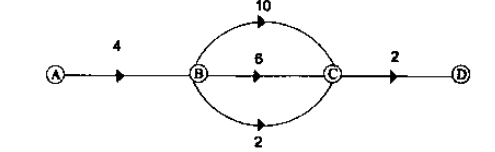
\includegraphics[width=0.4\columnwidth]{figs/43.png}
  \caption{project network}
  \label{fig:43}
\end{figure}
\begin{multicols}{4}
\begin{enumerate}
\item $15000$
\item $14000$
\item $13000$
\item $ 12000$
\end{enumerate}
\end{multicols}

\item A steel wire rope of diameter $25\,\mathrm{mm}$ weighing $37\,\mathrm{N/m}$ has $6$ strands of $7$ wires each. 
The diameter and tensile strength of each wire are $2.5\,\mathrm{mm}$ and $1800\,\mathrm{MPa}$, respectively. The factor of safety for raising a cage of weight $60\,\mathrm{kN}$ from a depth of $200\,\mathrm{m}$ is

\hfill\brak{GATE\ MN\ 2010}
\begin{multicols}{4}
\begin{enumerate}
\item $5.60$
\item $4.50$
\item $25$
\item $4.15$
\end{enumerate}
\end{multicols}

\item In block caving operation the draw points are placed at $20$ m center to center, with the pillar width
$3.5$ m as shown in the figure below. The muck is assumed to have zero cohesion and $35^\circ$ friction angle. The height of draw cone (h) in m is

\hfill\brak{GATE\ MN\ 2010}
\begin{figure}[H]
  \centering
  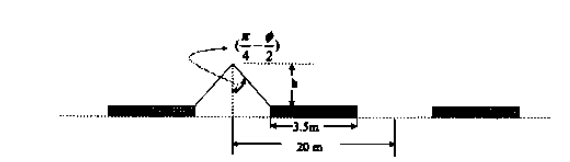
\includegraphics[width=0.4\columnwidth]{figs/45.png}
  \caption{block caving}
  \label{fig:45}
\end{figure}
\begin{multicols}{4}
\begin{enumerate}
\item $12.5 $
\item $14.6$
\item $15.8$
\item $ 16.5$
\end{enumerate}
\end{multicols}

\item The stroke length and pitch of the rifle bar of a percussive drill machine are $60$ mm and $\frac{1}{760}$ respectively. If the drill operates at $2000$ blows/minute, the rotational speed in rpm of the drill steel is

\hfill\brak{GATE\ MN\ 2010}
\begin{multicols}{4}
\begin{enumerate}
\item $145$
\item $158$
\item $162$
\item $175$
\end{enumerate}
\end{multicols}

\item The main fan operating point of a ventilation system is shown in the figure below. If an NPV of $200$ Pa assists the ventilation system, the resultant pressure \brak{Pa} and quantity \brak{m} generated by the fan respectively are

\hfill\brak{GATE\ MN\ 2010}
\begin{figure}[H]
  \centering
  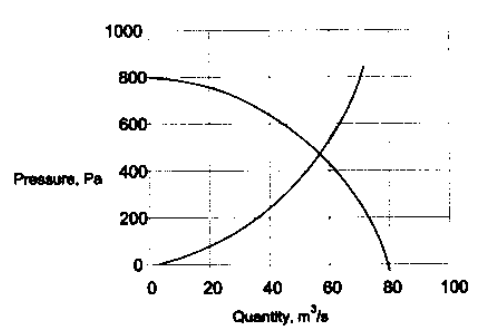
\includegraphics[width=0.4\columnwidth]{figs/graph47.png}
  \caption{Graphical representation }
  \label{fig:graph47}
\end{figure}
\begin{multicols}{4}
\begin{enumerate}
\item $500,68$
\item $600,63$
\item $640,55$
\item $400,63$
\end{enumerate}
\end{multicols}

\section*{Common Data Questions}
\subsection*{Common Data for Questions $48$ and $49$ $\colon$}
 The granular media in an ore bin is assumed to be of regular spherical shape, represented by the geometry as shown in the figure. The unit weight of solids is $25\ \text{kN/m}^3$.
\begin{figure}[H]
  \centering
  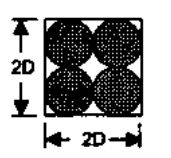
\includegraphics[width=0.2\columnwidth]{figs/4849.png}
  \caption{common data questions for Q48 and Q49}
  \label{fig:4849}
\end{figure}
\item The void ratio is


\hfill\brak{GATE\ MN\ 2010}
\begin{multicols}{4}
\begin{enumerate}
\item $0.91$
\item $0.84$
\item $0.78$
\item $0.69$
\end{enumerate}
\end{multicols}

\item The dry density in $\text{kN/m}^3$is

\hfill\brak{GATE\ MN\ 2010}
\begin{multicols}{4}
\begin{enumerate}
\item $13.09$
\item $12.50$
\item $11.74$
\item $10.87$
\end{enumerate}
\end{multicols}

\section*{Common Data for Questions $50$ and $51$  $\colon$}
Match the elements of a simple curve as given in the figure below.
\begin{figure}[H]
  \centering
  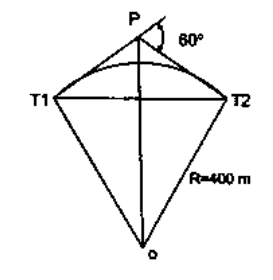
\includegraphics[width=0.4\columnwidth]{figs/5051.png}
  \caption{common data for Q50 and Q51}
  \label{fig:5051}
\end{figure}
\item The tangent length in m is


\hfill\brak{GATE\ MN\ 2010}

\begin{multicols}{4}
\begin{enumerate}
\item $215.5$
\item $220.4$
\item $228.4$
\item $230.9$
\end{enumerate}
\end{multicols}

\item The length of the long chord in m is


\hfill\brak{GATE\ MN\ 2010}

\begin{multicols}{4}
\begin{enumerate}
\item $375$
\item $400.0$
\item $415$
\item $450$
\end{enumerate}
\end{multicols}

\section*{Linked Answer Questions}
\subsection*{Statement for Linked Answer Questions $54$ and $55$ $\colon$}
A longwall panel with a face height of $3.0\ \text{m}$ and face length of $150.0\ \text{m}$ is worked in $3$ shifts per day employing $40$ men per shift. The depth of the web of the shearer cutting coal is $0.5\ \text{m}$. The unit weight of the coal is $1.4\ \text{tonne/m}^2$. Two full face cuts are executed per shift.
\item  The daily production from the panel in tonnes is


\hfill\brak{GATE\ MN\ 2010}

\begin{multicols}{4}
\begin{enumerate}
\item $945$
\item $1240$
\item $1890$
\item $2530$
\end{enumerate}
\end{multicols}

\item The panel OMS in tonnes is


\hfill\brak{GATE\ MN\ 2010}

\begin{multicols}{4}
\begin{enumerate}
\item $12.75$
\item $15.75$
\item $8.75$
\item $5.25$
\end{enumerate}
\end{multicols}

\subsection*{Statement for Linked Answer Questions $54$ and $55$ $\colon$}
Air at a density of $1.2\ \text{kg/m}^3$ flows in a straight duct such that the velocity at the centre is $12.5\ \text{m/s}$. The method factor for the velocity profile is known to be $0.80$.
\item The velocity pressure value in the duct in Pa is 


\hfill\brak{GATE\ MN\ 2010}
\begin{multicols}{4}
\begin{enumerate}
\item $31$
\item $47$
\item $60$
\item $83$
\end{enumerate}
\end{multicols}

\item  The air flow encounters a symmetric expansion such that the cross-sectional area of the duct becomes double. The static pressure value at the inlet and outlet of the expansion are $60$ Pa and $90$ Pa, respectively. Neglecting friction, the shock pressure loss on account of expansion in Pa is

\hfill\brak{GATE\ MN\ 2010}
\begin{multicols}{4}
\begin{enumerate}
\item $15$
\item $22$
\item $38$
\item $46$
\end{enumerate}
\end{multicols}

\section*{General Aptitude (GA) Questions}
\subsection*{Q.$56$-Q.$60$ carry one mark each.}
\item Which of the following options is the closest in meaning to the word below $\colon$
Exhert


\hfill\brak{GATE\ MN\ 2010}

\begin{enumerate}
\item urge
\item condemm
\item restrain
\item scold
\end{enumerate}

\item The question below consists of a pair of related words followed by four pairs of words. Select the
pair that best expresses the relation in the original pair.
\textbf{Preamble $\colon$ Constitution}


\hfill\brak{GATE\ MN\ 2010}

\begin{enumerate}
\item amendment $\colon$ law
\item prologue $\colon$ play
\item episode $\colon$ serial
\item plot $\colon$ story
\end{enumerate}

\item Choose the most appropriate word from the options given below to complete the following
sentence $\colon$
\textbf{The committee wrote a \underline{\hspace{1.5cm}} report, extolling only the strengths of the proposal.}


\hfill\brak{GATE\ MN\ 2010}

\begin{enumerate}
\item amendment $\colon$ law
\item prologue $\colon$ play
\item episode $\colon$ serial
\item plot $\colon$ story
\end{enumerate}

\item Choose the most appropriate word from the options given below to complete the following
sentence $\colon$
\textbf{If the country has to achieve real prosperity, it is \underline{\hspace{1.5cm}} that the frults of progress reach all, and in equal measure.}


\hfill\brak{GATE\ MN\ 2010}

\begin{enumerate}
\item inevitable
\item contingent
\item oblivious
\item imperative
\end{enumerate}

\item A person invests Rs.$1000$ at $10$\% annual compound interest for 2 years. At the end of two years the
whole amount is invested at an annual simple interest of $12$\% for $5$ years. The total value of the
investment finally is $\colon$


\hfill\brak{GATE\ MN\ 2010}

\begin{multicols}{4}
\begin{enumerate}
\item $1776$
\item $1760$
\item $1920$
\item $1936$
\end{enumerate}
\end{multicols}


\subsection*{Q.$61$-Q.$65$ carry two marks each.}
\item \textbf{The ban on smoking in designated public places can save a large mumber of people from the
well known effects of environmental tobacco smoke. Passive smoking seriously impairs respiratory health. The ban rightly seeks to protect non-smokers from its ill effects.}
Which of the following statements best sums up the meaning of the above passage $\colon$


\hfill\brak{GATE\ MN\ 2010}

\begin{enumerate}
\item Effects of environmental tobacco are well known.
\item The ban on smoking in public places protects the non smokers.
\item Passive smoking is bad for health
\item The ban on smoking in public places excludes passive smoking.
\end{enumerate}

\item Given the sequence A, B, B, C, C, C, D, D, D, D, $\ldots$ etc., that is one A, two Bs, three Cs, four Ds, five Es and so on, the $240^{\text{th}}$ letter in the sequence will be $\colon$
\hfill\brak{GATE\ MN\ 2010}
\begin{multicols}{4}
\begin{enumerate}
\item V
\item U
\item T
\item W
\end{enumerate}
\end{multicols}


\item Consider the set of integers $\{1, 2, 3, \ldots, 5000\}$. The number of integers that is divisible by neither $3$ nor $4$ is $\colon$


\hfill\brak{GATE\ MN\ 2010}

\begin{multicols}{4}
\begin{enumerate}
\item $1668$
\item $2084$
\item $2500$
\item $2916$
\end{enumerate}
\end{multicols}

\item A positive integer $m$ in base 10, when represented in base 2 has the representation $p$, and in base 3 has the representation $q$. We get $p - q = 990$, where the subtraction is done in base 10. Which of the following is necessarily true $\colon$

\hfill\brak{GATE\ MN\ 2010}

\begin{multicols}{4}
\begin{enumerate}
\item \(m \ge 14\)
\item \(9 \le m \le 13\)
\item \(6 \le m \le 8\)
\item \(m < 6\)
\end{enumerate}
\end{multicols}

\item Given the following four functions $\colon$ 
$f_1 $\brak{n}$= n^{100}$, 
$f_2 $\brak{n}$ = (1.2)^n$, 
$f_1 $\brak{n}$ = 2^{n/2}$, 
$f_1 $\brak{n}$ = 3^{n/3}$, 
which function will have the largest value for sufficiently large values of $n$ $\brak{\text{i.e., } n \to \infty}$?

\hfill\brak{GATE\ MN\ 2010}

\begin{multicols}{4}
\begin{enumerate}
\item $f_4$
\item $f_3$
\item $f_2$
\item $f_1$
\end{enumerate}
\end{multicols}

\begin{center}
\Large\textbf{{END OF THE QUESTION PAPER}}
\end{center}
\end{enumerate}

\end{document}




